\chapter{QKD Post-Processing on Programmable Network Hardware}
\label{ch:qkd-dpu}

\section{Principles of Quantum Key Distribution}
\label{sec:qkd-dpu-principles}

Quantum Key Distribution (QKD) leverages the fundamental principles of quantum mechanics---specifically, the no-cloning theorem and the observer effect---to establish a shared, secret cryptographic key between two parties, typically referred to as Alice and Bob~\cite{Xu2020}. Unlike classical public-key cryptography, which relies on the presumed computational hardness of mathematical problems, QKD provides information-theoretic security. Any attempt by an eavesdropper (Eve) to measure the quantum states in transit unavoidably disturbs them, introducing detectable errors. By monitoring the quantum bit error rate (QBER), Alice and Bob can upper-bound the information leaked to Eve and distill a perfectly secure key through classical post-processing.

QKD protocols fall into two primary paradigms (Figure~\ref{fig:qkd-paradigms}), distinguished chiefly by \emph{where the photon source sits and how much it must be trusted}:
\begin{itemize}
    \item \textbf{Prepare-and-Measure Protocols:} Here Alice hosts a \emph{trusted} source, encoding random bits in randomly chosen non-orthogonal bases and sending the photons to Bob, who measures in randomly chosen bases. The original BB84 protocol~\cite{bennett1984quantum} is the canonical example; its bit-level mechanics and classical post-processing are described in detail in Section~\ref{sec:qkd-dpu-bb84}, where BB84 underlies the post-processing pipeline studied in this chapter.
    \item \textbf{Entanglement-Based Protocols:} Pioneered by Ekert in 1991 (the E91 protocol)~\cite{ekert1991quantum}, these schemes distribute pairs of entangled photons from a central source that \emph{need not be trusted}. Such protocols allow for the source to be hosted by a third party (often called Charlie) who sends one photon to Alice and one to Bob. Security is certified directly from the measured data by a Bell-inequality test: a Bell parameter $S$ exceeding its classical bound of $2$ proves the photons are genuinely entangled and uncorrelated with any classical variable held by an eavesdropper, and the magnitude of the violation bounds the information available to that eavesdropper.
\end{itemize}

\begin{figure}[htbp]
  \centering
  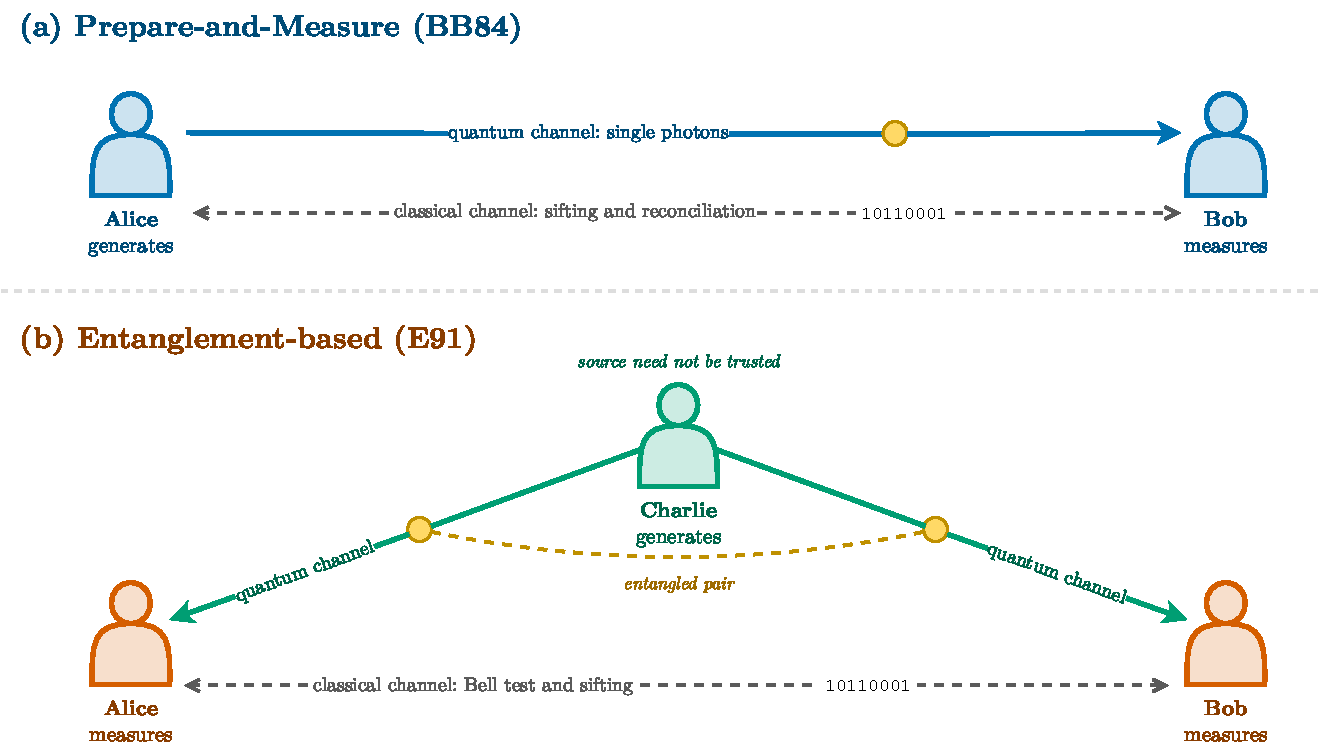
\includegraphics[width=\linewidth]{figures/chapter4/qkd_paradigms.pdf}
  \caption{The two principal QKD paradigms differ in where the photon source
  sits and how much it must be trusted. In \textbf{(a)} prepare-and-measure
  (BB84), Alice hosts a \emph{trusted} source, preparing photons in randomly
  chosen non-orthogonal bases and sending them to Bob over a quantum channel;
  basis sifting and reconciliation proceed over a classical channel. In
  \textbf{(b)} entanglement-based QKD (E91), a central party (Charlie) operates
  a source that \emph{need not be trusted}, distributing one photon of each
  entangled pair to Alice and one to Bob; security is instead certified by a
  Bell-inequality test ($S>2$), so genuine entanglement---rather than trust in
  the source---guarantees secrecy. In both paradigms, Alice and Bob exchange
  basis and reconciliation information over an authenticated classical channel
  and distil a shared secret key (matching bit strings); any eavesdropping on
  the quantum channel raises the quantum bit error rate (QBER) and is thereby
  detectable.}
  \label{fig:qkd-paradigms}
\end{figure}

Entanglement-based schemes are particularly crucial for the vision of a quantum internet~\cite{Wehner2018}. They enable device-independent QKD and supply the entanglement resource on which quantum teleportation and entanglement swapping rely---the primitives that, in the quantum repeaters of Section~\ref{sec:qsrc-distance}, route quantum states across multi-hop topologies rather than over single point-to-point links.

\section{The BB84 Protocol and Raw Key Generation}
\label{sec:qkd-dpu-bb84}

To understand the computational burden of QKD, it is necessary to first examine how raw key material is generated. The prototypical example is the BB84 protocol~\cite{bennett1984quantum}, a prepare-and-measure scheme that serves as the foundation for the synthetic quantum source evaluated in this chapter.

In BB84, Alice seeks to share a secret key with Bob. She generates a sequence of random classical bits and encodes each into a single photon. While nearly every textbook renders BB84 using $\uparrow\!\rightarrow\!\nearrow\!\searrow$ arrows denoting polarization encoding, we take the road less travelled here and carry the bits in the photon's \emph{frequency} (spectral) degree of freedom instead, aligning with the states produced by the quantum sources of Chapter~\ref{ch:quantum-sources}. BB84 is agnostic to the physical carrier: any pair of mutually unbiased bases suffices.

For each bit, Alice randomly chooses one of two such bases. In the frequency basis ($f$) she localizes the photon in one of two discrete frequency bins, encoding a `0` as $|f_0\rangle$ and a `1` as $|f_1\rangle$. In the phase basis ($\phi$) she instead prepares an equal superposition of the two bins, encoding a `0` as $|{+}\rangle$ and a `1` as $|{-}\rangle$, where $|{\pm}\rangle = (|f_0\rangle \pm |f_1\rangle)/\sqrt{2}$ are the two bins combined with relative phase $\varphi=0$ and $\varphi=\pi$, respectively.

Alice transmits this stream of single photons to Bob over a quantum channel, such as a dedicated optical fiber. Upon receiving a photon, Bob must measure its state to recover the bit. However, because he does not know which basis Alice used, he randomly and independently chooses a measurement basis ($f$ or $\phi$) for each incoming photon: the frequency basis is read out by a filter that resolves which bin the photon occupies, while the phase basis requires electro-optically mixing the two bins before detection so that their relative phase becomes measurable.

If Bob guesses the same basis Alice used, quantum mechanics guarantees he will measure the correct bit (in an ideal, noiseless system). If he guesses the wrong basis, his measurement result is completely uncorrelated with Alice's original bit. Furthermore, the no-cloning theorem prevents an eavesdropper, Eve, from copying the photons to measure later. If Eve attempts to intercept and measure the photons in transit, her own random basis choices will inevitably disturb the quantum states, introducing a detectable error rate into the channel.

The quantum transmission concludes with Alice and Bob each holding a string of bits (Bob's measurements and Alice's original bits) and a corresponding array of the bases they used. Table~\ref{tab:bb84-sifting} traces this process over a short sequence of rounds, showing how only the rounds in which their independently chosen bases happen to agree survive into the sifted key. At this point, the quantum physical layer's job is complete. However, this raw key is entirely unusable for cryptography: it is riddled with errors from basis mismatches, optical channel noise, and potential eavesdropping.

\begin{table}[htbp]
  \centering
  \caption{A worked BB84 example over eight transmission rounds, using
  frequency-bin rather than the customary polarization encoding. Alice encodes
  each random bit in a randomly chosen basis---the frequency basis
  ($f$: $|f_0\rangle$ for~0, $|f_1\rangle$ for~1) or the phase basis
  ($\phi$: $|{+}\rangle$ for~0, $|{-}\rangle$ for~1, with
  $|{\pm}\rangle=(|f_0\rangle\pm|f_1\rangle)/\sqrt{2}$)---and Bob measures in his
  own randomly chosen basis. When the bases agree, Bob recovers Alice's bit;
  when they disagree, his outcome is uncorrelated ($-$) and the round is
  discarded during sifting. The surviving bits form the raw sifted key, from
  which errors are still removed by the classical post-processing pipeline of
  Section~\ref{sec:qkd-dpu-bottleneck}.}
  \label{tab:bb84-sifting}
  \begin{tabular}{l*{8}{c}}
    \toprule
    Round & 1 & 2 & 3 & 4 & 5 & 6 & 7 & 8 \\
    \midrule
    Alice's bit          & 0 & 1 & 1 & 0 & 1 & 0 & 0 & 1 \\
    Alice's basis        & $f$ & $\phi$ & $f$ & $\phi$ & $f$ & $\phi$ & $f$ & $\phi$ \\
    State sent           & $|f_0\rangle$ & $|{-}\rangle$ & $|f_1\rangle$ & $|{+}\rangle$ & $|f_1\rangle$ & $|{+}\rangle$ & $|f_0\rangle$ & $|{-}\rangle$ \\
    Bob's basis          & $f$ & $f$ & $f$ & $\phi$ & $\phi$ & $\phi$ & $\phi$ & $\phi$ \\
    Bob's bit            & 0 & $-$ & 1 & 0 & $-$ & 0 & $-$ & 1 \\
    \midrule
    Bases agree?         & \checkmark & $\times$ & \checkmark & \checkmark & $\times$ & \checkmark & $\times$ & \checkmark \\
    Sifted key           & 0 & & 1 & 0 & & 0 & & 1 \\
    \bottomrule
  \end{tabular}
\end{table}

\section{The Computational Bottleneck of Post-Processing}
\label{sec:qkd-dpu-bottleneck}

To transform this error-riddled raw key into a secure, usable cryptographic key, Alice and Bob must execute a classical post-processing pipeline. While the physical generation, transmission, and detection of quantum states (as discussed in Chapter~\ref{ch:quantum-sources}) have seen tremendous advancements, executing this classical pipeline at scale introduces a significant computational load. This pipeline consists of several computation-heavy stages:

\begin{enumerate}
    \item \textbf{Sifting:} Alice and Bob exchange their basis choices over an authenticated classical channel and discard measurements where incompatible bases were used.
    \item \textbf{Error Estimation:} A subset of the sifted bits is publicly compared to estimate the quantum bit error rate (QBER). Because the protocol assumes all errors are caused by an eavesdropper, the QBER bounds the maximum information Eve could have gained.
    \item \textbf{Information Reconciliation:} To resolve discrepancies between Alice's and Bob's strings caused by channel noise, the parties perform forward error correction. This is typically achieved using rate-adaptive Low-Density Parity-Check (LDPC) codes or the Cascade protocol. For LDPC, the receiver executes iterative belief propagation (e.g., the min-sum algorithm) to converge on the correct string.
    \item \textbf{Privacy Amplification:} Once the strings match, Alice and Bob compress them using a universal hash function (such as Toeplitz matrix multiplication) to erase any partial information the eavesdropper might hold, yielding the final, perfectly secret key.
\end{enumerate}

The computational complexity of this pipeline is substantial, particularly during information reconciliation and privacy amplification. As the QBER rises due to optical channel impairments or distance, LDPC decoding requires larger matrices, more iterations, and lower code rates, scaling the computational burden exponentially. Furthermore, all classical communication during these steps must be strictly authenticated to prevent man-in-the-middle attacks.

\section{Programmable Network Hardware and the Trust Boundary}
\label{sec:qkd-dpu-trust}

Datacenter networks operate at terabit-per-second scales, relying heavily on low-latency, high-throughput transport protocols. Traditionally, QKD post-processing has been executed either on rigid FPGA appliances or on general-purpose host CPUs. Both integration models suffer from structural flaws when deployed in high-performance environments.

Dedicating host CPU cycles to cryptographic key distillation becomes economically and operationally prohibitive. Executing iterative LDPC belief propagation and large-scale Toeplitz hashing on x86 processors consumes the compute resources the datacenter is built to provide. Alternatively, offloading these tasks to a standalone FPGA appliance solves the compute bottleneck but fragments the trust boundary: the distilled key must still be securely transported from the appliance to the server's network interface card (NIC) where the actual data encryption takes place. Whether using an external Key Management System (KMS) or transferring the keys across the host's PCIe bus, this handoff adds latency, restricts key-injection throughput, and exposes the plaintext key material to potential software or bus vulnerabilities.

This chapter proposes and evaluates an architecture that collapses the key generation and key consumption trust boundaries into a single network device. By offloading the entire post-processing pipeline to the Arm cores of an NVIDIA BlueField-3 Data Processing Unit (DPU), the architecture isolates the key material from the host CPU. The DPU natively performs sifting, LDPC error correction, and privacy amplification, ensuring the host CPU utilization remains at zero.

\section{Quantum-Secured Datacenter Fabrics (Q-RDMA)}
\label{sec:qkd-dpu-rdma}

The primary motivation for offloading QKD to the DPU is to protect latency-sensitive datacenter workloads without degrading their performance. Modern distributed training clusters, storage backends, and high-frequency trading platforms rely on Remote Direct Memory Access (RDMA) over Converged Ethernet (RoCEv2) to bypass the host kernel and achieve microsecond latencies.

Standard, software-based encryption fundamentally breaks RDMA by forcing traffic back through the host's CPU and memory subsystem. To securely encrypt RDMA, the cryptography must be applied inline by the network hardware.

By executing QKD post-processing entirely within the DPU, the resulting quantum-secure keys never cross the PCIe bus to the host. Instead, they are formatted as Security Associations (SAs) and injected seamlessly into the DPU's local hardware IPsec or MACsec encryption engines. This enables quantum-secured RDMA (Q-RDMA). The data plane encryption operates transparently at line rate, while the continuous distillation of fresh keys occurs asynchronously on the DPU's Arm cores. Consequently, the fabric's latency and throughput remain completely isolated from the heavy computational cost of QKD key generation. To evaluate this architecture under stable, reproducible error conditions---rather than at the mercy of the environmental drift, dark counts, and afterpulsing that plague physical optical hardware---the included paper emulates the qubit transmission layer with a synthetic BB84 source that injects controlled QBER profiles, while running the entire post-processing pipeline, key derivation, and hardware IPsec injection on real BlueField-3 silicon.

\section{Contribution and Articles}
\label{sec:qkd-dpu-context}

This chapter is built around one contribution (P3), the manuscript \enquote{QKD Post-Processing Offload on BlueField-3 DPUs: Towards Quantum-Secured RDMA in Datacenter Fabrics}.

This manuscript was accepted and presented at IEEE Quantum Week (QCE). The paper contributes a complete hardware/software co-design strategy for offloading the classical communication channel, LDPC decoding, and IPsec key injection onto a DPU. This demonstrates that continuous distillation of fresh keys can occur asynchronously on programmable network hardware without burdening the host CPU.

Beyond this article, the work on quantum-secured networking also contributed to several filed patent applications, \enquote{Multi-Hybrid Cryptographic Key Exchange (MHKE)} (I2) and \enquote{ROSE-QKD: Receiver-Only, Semi-Honest Emitter Quantum Key Distribution} (I3), together with a draft application on \enquote{Capability-Based Authentication of Quantum Nodes via Statistical Analysis} (I4). These inventions, which extend the architectural concepts evaluated in this chapter, are reported at title level among the patents in the List of Publications.

This paper addresses the core integration challenge outlined in \textbf{RQ2}: how to make QKD systems scalable and practical in high-performance datacenters. It closes the gap between quantum key generation (explored in Chapter~\ref{ch:quantum-sources}) and deployable datacenter security by offloading the full post-processing pipeline---sifting, error estimation, reconciliation, and privacy amplification---onto a BlueField-3 DPU. By injecting the distilled keys directly into the DPU's hardware encryptors, quantum-secured RDMA retains line-rate latency and throughput.

\includedpaper{P3}{QKD Post-Processing Offload on BlueField-3 DPUs: Towards Quantum-Secured RDMA in Datacenter Fabrics}{meyer2026qkd}{source-materials/papers/camera-ready/QKD_PostProc_DPUs.pdf}

\section{Discussion and Transition}

While QKD offers information-theoretic security for key distribution, it requires specialized optical hardware and dedicated fiber links, making it challenging to deploy ubiquitously across all network segments. To achieve comprehensive quantum-safe security, QKD must be complemented by PQC---classical cryptographic algorithms believed to be secure against quantum computers. The next chapter explores this complementary approach, shifting the focus from quantum-generated security material to the execution of PQC algorithms on the same programmable network infrastructure used here for QKD post-processing.
